\documentclass[10pt,a4paper,french]{article}
\author{par Léo Peyronnet}
\title{Interpolation et Approximation}
\date{Novembre 2022}

\usepackage[utf8]{inputenc}
\usepackage[T1]{fontenc}

\usepackage{babel}
\usepackage{listings}
\usepackage{amsfonts}
\usepackage{amsmath}
\usepackage{amssymb}
\usepackage{amsthm}
\usepackage{mathtools}
\usepackage{tabto}
\usepackage{color}
\usepackage[table]{xcolor}

\lstset{
  aboveskip=3mm,
  belowskip=-2mm,
  basicstyle=\footnotesize,
  breakatwhitespace=false,
  breaklines=true,
  captionpos=b,
  commentstyle=\color{red},
  deletekeywords={...},
  escapeinside={\%*}{*)},
  extendedchars=true,
  framexleftmargin=16pt,
  framextopmargin=3pt,
  framexbottommargin=6pt,
  frame=tb,
  keepspaces=true,
  keywordstyle=\color{blue},
  language=C,
  literate=
  {²}{{\textsuperscript{2}}}1
  {⁴}{{\textsuperscript{4}}}1
  {⁶}{{\textsuperscript{6}}}1
  {⁸}{{\textsuperscript{8}}}1
  {€}{{\euro{}}}1
  {é}{{\'e}}1
  {è}{{\`{e}}}1
  {ê}{{\^{e}}}1
  {ë}{{\¨{e}}}1
  {É}{{\'{E}}}1
  {Ê}{{\^{E}}}1
  {û}{{\^{u}}}1
  {ù}{{\`{u}}}1
  {â}{{\^{a}}}1
  {à}{{\`{a}}}1
  {á}{{\'{a}}}1
  {ã}{{\~{a}}}1
  {Á}{{\'{A}}}1
  {Â}{{\^{A}}}1
  {Ã}{{\~{A}}}1
  {ç}{{\c{c}}}1
  {Ç}{{\c{C}}}1
  {õ}{{\~{o}}}1
  {ó}{{\'{o}}}1
  {ô}{{\^{o}}}1
  {Õ}{{\~{O}}}1
  {Ó}{{\'{O}}}1
  {Ô}{{\^{O}}}1
  {î}{{\^{i}}}1
  {Î}{{\^{I}}}1
  {í}{{\'{i}}}1
  {Í}{{\~{Í}}}1,
  morekeywords={*,...},
  numbers=left,
  numbersep=10pt,
  numberstyle=\tiny\color{black},
  rulecolor=\color{black},
  showspaces=false,
  showstringspaces=false,
  showtabs=false,
  stepnumber=1,
  stringstyle=\color{gray},
  tabsize=4,
  title=\lstname,
}

\begin{document}
\maketitle
Compte rendu du TP consistant à programmer et comparer certaines méthodes d'interpolation et d'approximation.
\section{Rappel des méthodes}
\subsection{Méthodes d'interpolations}
L'interpolation est une opération mathématique visant à déterminer une fonction passant par des points donnés du plan. Plus précisément, soient $x_1,...,x_n$ des réels distincts, $y_1,...,y_n$ des réels, $n \in \mathbb{N^*}$. Alors l'interpolation consiste à déterminer une fonction telle que $\forall i \in [1,n],f(x_i)=y_i$; ce qui correspond à passer par l'ensemble des points d'interpolations $(x_i,y_i)$.

Les méthodes détaillés ci-dessous interpolent des fonctions polynomiales de degré au plus $n-1$.
\subsubsection{Méthode de Lagrange}
La méthode de Lagrange se base sur le principe de superposition, c'est à dire que les points d'interpolation vont être traités un par un.

Soit $L_1,...,L_n \in \mathbb{R}_{(n-1)}[X]$ tels que $\forall a,b \in [1,n]$, $L_a(x_b)=1$ si $a=b$, $0$ sinon, alors le polynôme $P_{(n-1)}$ est exprimé sous la forme:
\begin{align*}
P_{(n-1)}(x)=\sum_{i=0}^{(n-1)}y_i L_i(x)
\end{align*}
avec $L_i(x)$:
\begin{align*}
L_i(x)=\prod_{j=0,j\neq i}^{(n-1)}\frac{x-x_j}{x_i-x_j}
\end{align*}
\subsubsection{Méthode de Neville}
Quant à elle, la méthode de Neville se base sur la décomposition du polynome $P_{(n-1)}[x_1,x_2,...,x_n]$ en $P_{(n-2)}[x_1,x_2,...,x_{n-1}]$ et $P_{(n-2)}[x_2,x_3,...,x_{n}]$, et ainsi de suite.

Alors, en admettant $P_0[x_i],\forall x,i=0,...,n-1 ; P_0[x_i](x)=y_i$:
{\tiny
\begin{align*}
&\forall x,P_{k}[x_i,...,x_{i+k}](x)=\frac{(x-x_{i+k})P_{k-1}[x_i,...,x_{i+k-1}](x)+(x_i-x)P_{k-1}[x_i+1,...,x_{i+k}](x)}{x_i-x_{i+k}},\\&\forall k=1,...,n-1
\end{align*}
}
\section{Présentation des programmes}
\subsection{lagrange()}
\begin{lstlisting}
float lagrange(float * X,float * Y,float xentree, int taille){
    float result=0;
    for (int i=0;i<taille;i++){ //boucle i
        float Li=1;
        for (int j=0;j<taille;j++){ //boucle j
            if (j!=i){
                Li*=(xentree-X[j])/(X[i]-X[j]); //produit
            }
        }  
        result+=Y[i]*Li; //somme des produits par Y[i]
    }
    return result;
}
\end{lstlisting}
La boucle $j$ correspond à l'opérateur produit, la boucle $i$ correspond à l'opérateur somme.\\
Complexité temporelle: $o(x^2)$.
\subsection{neville()}
\begin{lstlisting}
double neville(float * X,float * Y,float xentree, int n){
    double * Pk=(double *)malloc(n * sizeof(double));
    if (Pk==NULL){return 0;}
    for (int j=0;j<n;j++){
        Pk[j]=Y[j]; //Initialisation de P_0
    }

    for(int k=1;k<n;k++){
        for(int i=0;i<n;i++){
            Pk[i]=((xentree-X[i+k])*Pk[i]+(X[i]-xentree)*Pk[i+1])/(X[i]-X[i+k]);
        }
    }
    return Pk[0];
}

\end{lstlisting}
La boucle $j$ permet d'initialiser $P_0$ tel que défini plus haut. Les boucles $k$ et $i$ correspondent aux variables définies plus haut. L'utilisation de variables "double" plutôt que de simples "float" sera détaillé plus tard. (c.f.: \ref{double})\\
Complexité temporelle: $o(x^2)$.
\subsection{Fonctions de conformité}
Fonctions propres à chacune des méthodes d'interpolation pour s'assurer de l'adéquation du polynôme interpolé aux jeux d'essais proposés, c'est à dire si $f(x)=y$. 

Les fonctions affichent leurs résultats dans le terminal pour chaque point du jeu de données et renvoie 0 si le polynôme est conforme pour l'ensemble du jeu de données, sinon un entier $n\in \{1,...,t\}$, avec $t$ le nombre de points dans le jeu. 
\subsubsection{conformLagrange()}
\begin{lstlisting}
int conformLagrange(float * X,float * Y, int taille){
    int result=0;
    for (int i=0;i<taille;i++){
        printf("lagrange(%g)==Y[%d]: ",X[i],i);
        if(lagrange(X,Y,X[i],taille)==Y[i]){ //f(x)=y ?
            printf("True\n");
        }
        else{
            printf("False\n");
            result++;
        }
    }
    return result;
}
\end{lstlisting}
\subsubsection{conformNeville()}\label{double}
\begin{lstlisting}
int conformNeville(float * X,float * Y, int taille){
    int result=0;
    for (int i=0;i<taille;i++){
        printf("neville(%g)==Y[%d]: ",X[i],i);
        if(neville(X,Y,X[i],taille)==Y[i]){ //f(x)=y ?
            printf("True\n");
        }
        else{
            printf("False\n");
            result++;
        }
    }
    return result;
}
\end{lstlisting}
Le prédicat déterminant la conformité posait problème lorsque la valeur de retour de neville() était de simple précision, la passer en double précision régla le problème.
\section{Observations sur les jeux d'essais}
\subsection{Densité de l'eau en fonction de la température}

\begin{center}
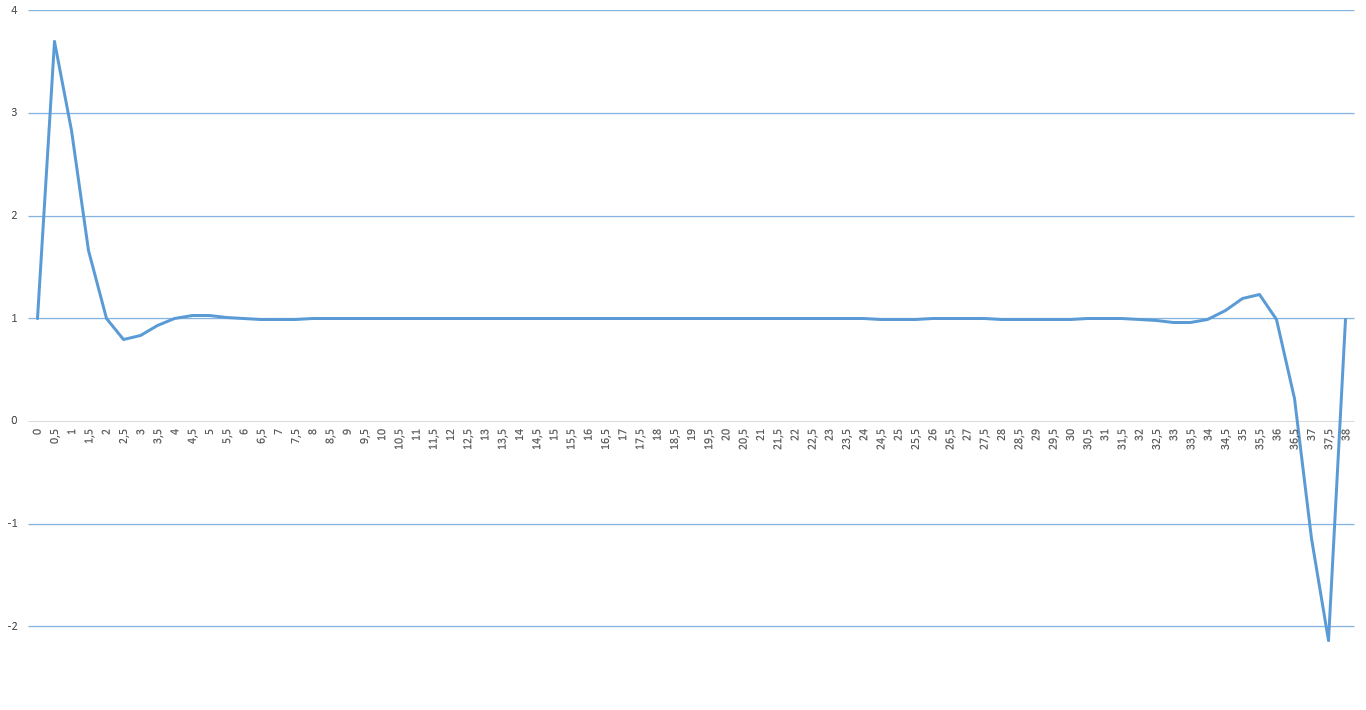
\includegraphics[scale=0.25]{ressources/lagrange_1.PNG}
\end{center}
\begin{center}
\textit{Méthode Lagrange: $x\in \{0,0.5,1,...,38\}$ }
\end{center}

\begin{center}
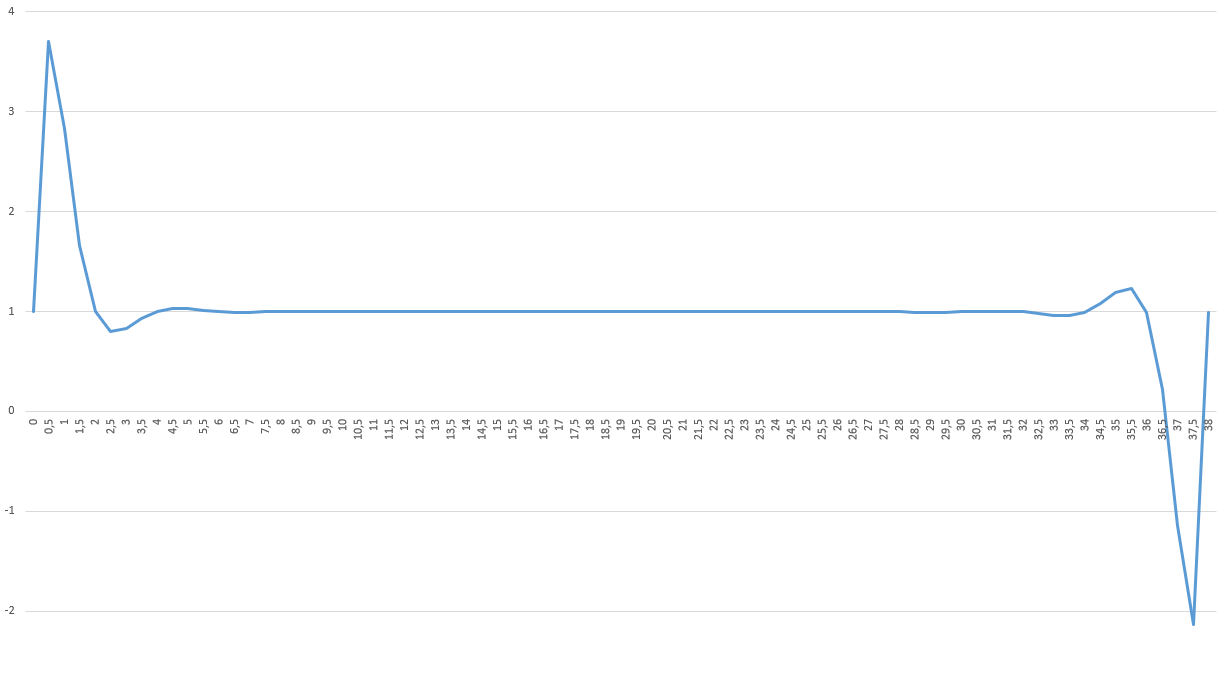
\includegraphics[scale=0.25]{ressources/neville_1.PNG}
\end{center}
\begin{center}
\textit{Méthode Neville: $x\in \{0,0.5,1,...,38\}$ }
\end{center}

\subsection{Dépenses mensuelles et revenus}

\begin{center}
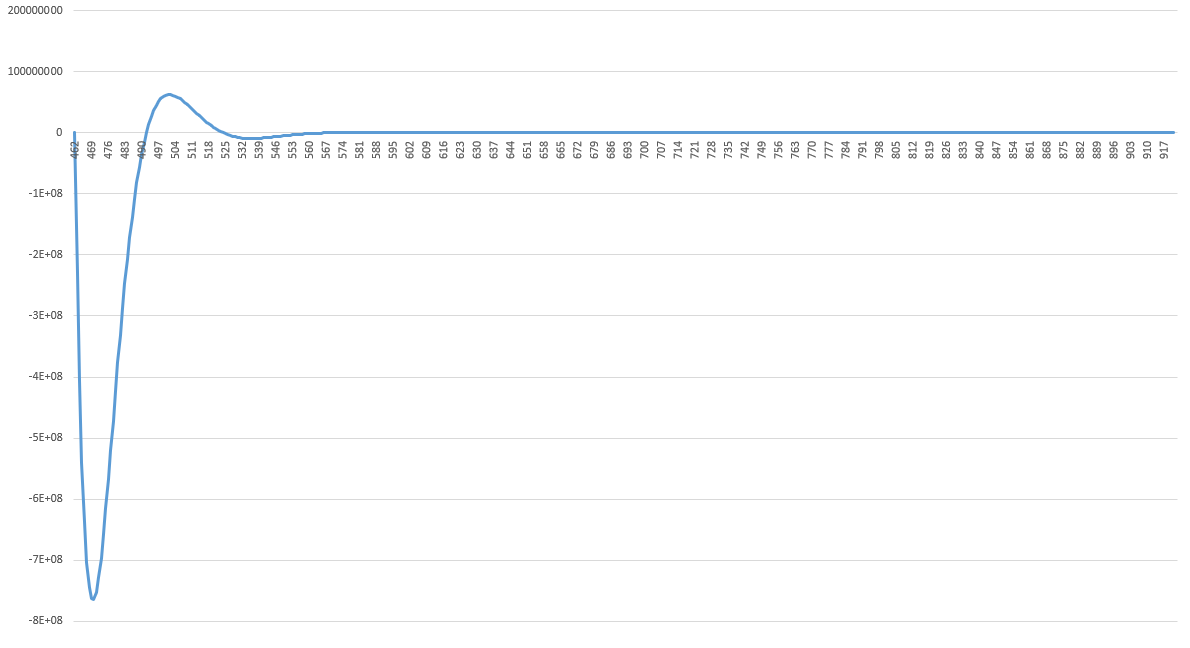
\includegraphics[scale=0.25]{ressources/lagrange_2.PNG}
\end{center}
\begin{center}
\textit{Méthode Lagrange: $x\in \{462,463,464,...,921\}$ }
\end{center}

\begin{center}
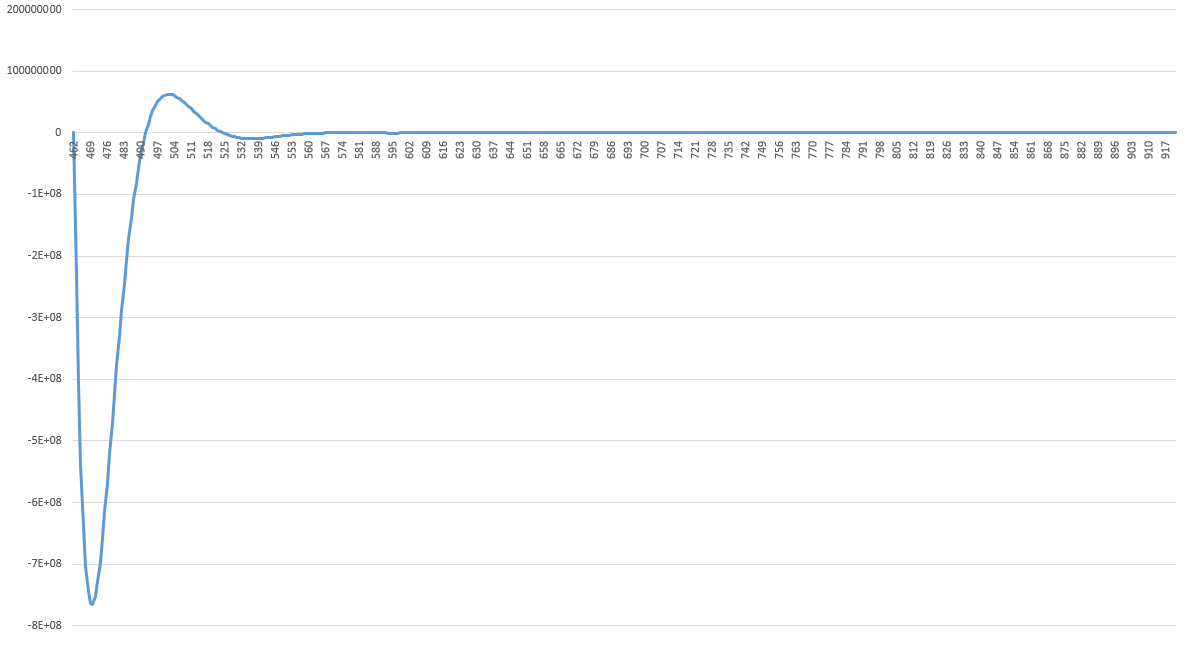
\includegraphics[scale=0.25]{ressources/neville_2.PNG}
\end{center}
\begin{center}
\textit{Méthode Neville: $x\in \{462,463,464,...,921\}$ }
\end{center}

\subsection{Série S due à Anscombe}

\begin{center}
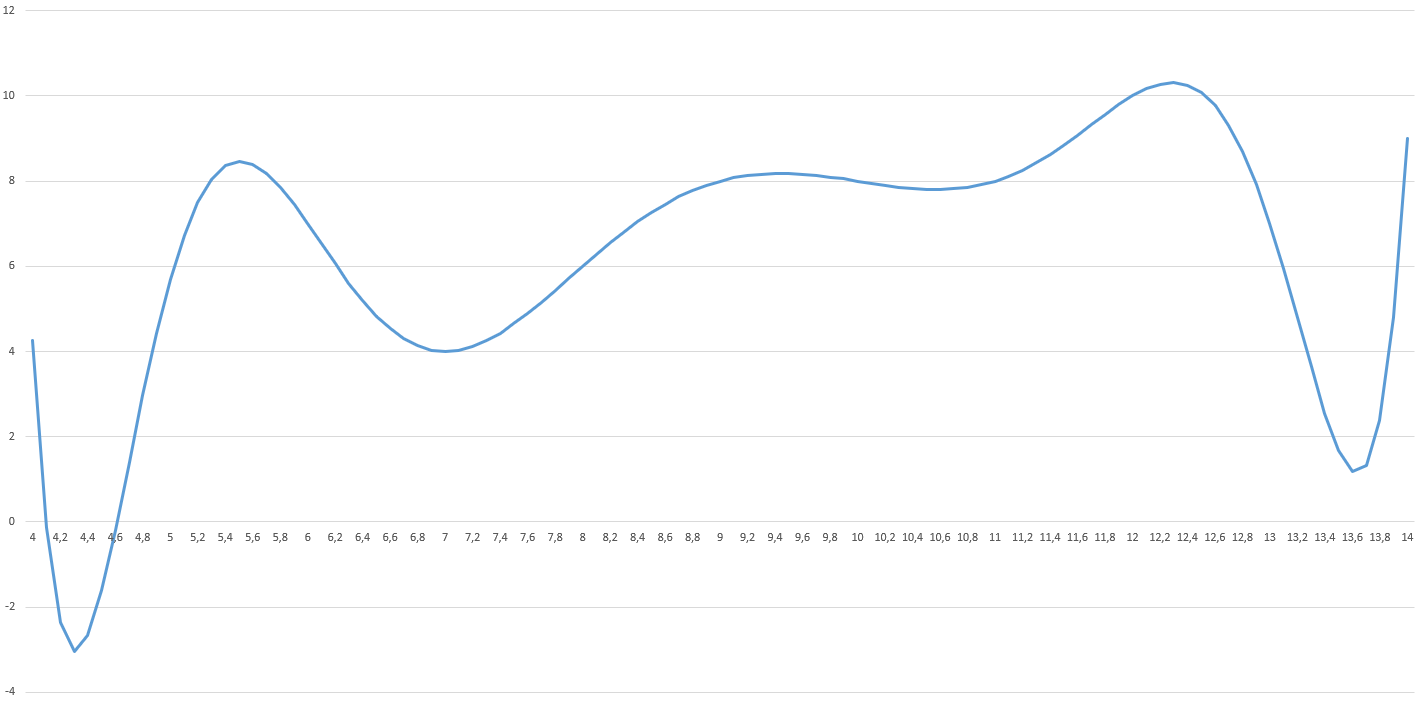
\includegraphics[scale=0.25]{ressources/lagrange_3.PNG}
\end{center}
\begin{center}
\textit{Méthode Lagrange: $x\in \{4,4.1,4.2,...,14\}$ }
\end{center}

\begin{center}
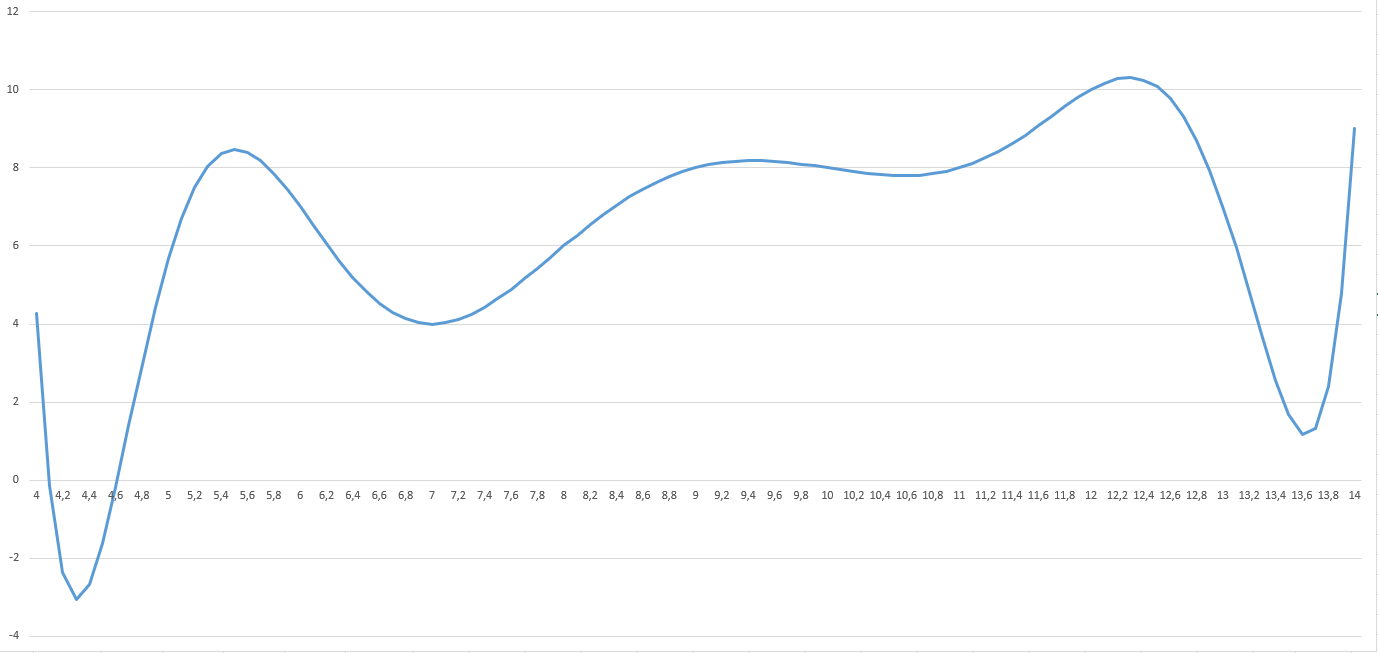
\includegraphics[scale=0.25]{ressources/neville_3.PNG}
\end{center}
\begin{center}
\textit{Méthode Neville: $x\in \{4,4.1,4.2,...,14\}$ }
\end{center}

\end{document}